\documentclass[a4paper,12pt]{article}

%Class
	%\documentclass[a4paper,12pt]{article}

%Packages
	\usepackage{amsmath}					% Standard maths
	\usepackage{amssymb}					% Standard maths
	\usepackage{amsthm}						% Standard maths
	\usepackage{thmtools, thm-restate}% Theorem styles
	\usepackage{mathtools}
	\usepackage[newzealand]{babel}% Date/time in British format (yes, I know it says NZ)
	\usepackage{datetime}					% Date/time
	\usepackage{multirow}					% For stacked subscripts
	\usepackage{xcolor}						% For colour!
	\usepackage[normalem]{ulem}		% For strikeout
	\usepackage{isomath}
	\usepackage{fancyhdr}					% For the headers
	\usepackage{mfirstuc}					% For the headers
	\usepackage[hmargin=1in,top=0.8in,bottom=1in]{geometry} % Page margins more reasonable
	\usepackage{graphicx}					% For including graphics
	%\usepackage{float}						% For something
	\usepackage{enumitem}					% For numbering tweaks
	\usepackage[margin=15pt,font={footnotesize},labelfont=bf,format=hang]{caption}
\usepackage[margin=15pt,font={footnotesize},labelfont=bf,format=hang]{subcaption}
	\usepackage{url}
	\usepackage[hidelinks]{hyperref}	% For hyperlinks
	\usepackage{breakurl}
	\usepackage{cleveref}
	\usepackage[scaled=.92]{helvet}
	\newbool{show_question}
	\newbool{show_solution}
	\newcommand{\solutioninheading}{\ifbool{show_solution}{: SOLUTIONS}{}}
	\usepackage{pgfplots}
\newcommand{\ep}{\varepsilon}

\makeatletter 
\newcommand\mynobreakpar{\par\nobreak\@afterheading} 
\makeatother

    \newcommand{\question}[3]{
    	\item \textbf{#1} \mynobreakpar \nobreak \medskip % Title
    	%
    	\ifbool{show_question}{\nobreak#2}{} % Question
    	%
    	%
    	\ifbool{show_question}{\ifbool{show_solution}{\par\medskip\textbf{Solution:}}{}}{} % Both
    	\ifbool{show_solution}{#3}{} % Answer
    }		

%MATHEMATICAL SHORTCUTS
%Two and three-part definitions
	\newcommand{\twopartdef}[4]
	{	\left\{
			\begin{array}{ll}
				#1 & \mbox{if } #2 \\
				#3 & \mbox{if } #4
			\end{array}
		\right.}
%	\newcommand{\threepartdef}[6]
%	{	\left\{
%			\begin{array}{ll}
%				#1 & \mbox{if } #2 \\
%				#3 & \mbox{if } #4 \\
%				#5 & \mbox{if } #6
%			\end{array}
%		\right.}
%Blackboard bold	
	\newcommand{\N}{{\mathbb N}} 
	\newcommand{\R}{{\mathbb R}} 
	\newcommand{\C}{{\mathbb C}} 
	%Curly letters
%	\newcommand{\E}{{\mathcal E}}	
%	\newcommand{\F}{{\mathcal F}} 
%	\newcommand{\Null}{{\mathcal N}} 
%	\newcommand{\R}{\mathcal{R}} 
%	\newcommand{\Z}{\mathcal{Z}} 
%Uprights
	\newcommand{\D}{{\mathrm D}}
	\renewcommand{\d}{{\mathrm d}}
%Easy Greeks
%	\def\a{\alpha}
%	\def\g{\gamma}
%	\newcommand{\e}{{\varepsilon}}
%	\newcommand{\la}{{\lambda}}  
%	\newcommand{\om}{{\Omega}}
	\renewcommand{\epsilon}{\varepsilon}
	
%Vector operators
	\def \p {\partial}
	\newcommand{\del}{{\nabla}}
	\newcommand{\grad}{{\nabla}}
    \newcommand{\vdel}{\boldsymbol{\nabla}}
    \newcommand{\vgrad}{\boldsymbol{\nabla}}
    \newcommand{\vnabla}{\boldsymbol{\nabla}}
	\newcommand{\cross}{{\times}}
	\newcommand{\Lap}{{\nabla^2}} 
%Arrows
%	\newcommand{\goesto}[1]{\xrightarrow[#1]{}}
%hats
%	\newcommand{\nhat}{\widehat{\v{n}}}
%	\newcommand{\shat}{\widehat{\v{s}}}
	\renewcommand{\hat}{\widehat}
%Note to self
%	\newcommand{\note}[1]{[\textbf{\textsl{\MakeUppercase{#1}}}]}
	
%Stress tensor
%	\newcommand{\T}{\vg{\sigma}}

% Vectors, quaternions etc.
\renewcommand{\v}[1]{\mathbfit{#1}}      % Generic vector
\newcommand{\vc}[1]{\bm{\mathcal{#1}}}      % vector mathcal
\newcommand{\uv}[1]{\widehat{\mathbfit{#1}}}      % Generic unit vector
\newcommand{\q}[1]{\mathsfbfit{#1}}        % Generic quaternion
\renewcommand{\t}[1]{\mathsfbfit{#1}}	 % Generic tensor
\newcommand{\m}[1]{\mathsfbfit{#1}}	 % Generic matrix
\newcommand{\vu}[1]{\mathbf{#1}}         % Upright vector (for zero vector)
\newcommand{\qu}[1]{\mathbf{#1}}       % Upright quaternion (for zero quaternion)
\newcommand{\tu}[1]{\bm{\mathsf{#1}}}	 % Upright tensor (for zero tensor)

%Real and imaginary
\renewcommand{\Re}{\operatorname{Re}}
\renewcommand{\Im}{\operatorname{Im}}
	
%Non-dim numbers
%	\renewcommand{\Re}{\operatorname{Re}}
%	\newcommand{\Bi}{\operatorname{Bi}}
%	\newcommand{\Fo}{\operatorname{Fo}}
	
%Misc
\DeclareMathSymbol{\Delta}{\mathalpha}{operators}{1} % Keeps Delta upright
\DeclareMathSymbol{\Gamma}{\mathalpha}{operators}{0} % Keeps Gamma upright
	\newcommand{\cosec}{\operatorname{cosec}}
	\newcommand{\cosech}{\operatorname{cosech}}
	\newcommand{\sech}{\operatorname{sech}}
	\newcommand{\tr}{\operatorname{tr}}
	\newcommand{\erf}{\operatorname{erf}}
	\newcommand{\order}{\mathcal{O}}
%	\newcommand{\V}{\mathcal{V}} % 	CurlyV = (Bi V) / (1 + Bi)

% Differentiating 
\newcommand{\fd}[2]{\mathchoice{\frac{\d #1}{\d #2}}{\d #1/\d #2}{\d #1/\d #2}{\d #1/\d #2}}
\newcommand{\fdd}[2]{\mathchoice{\frac{\d^2 #1}{\d #2^2}}{\d^2 #1/\d #2^2}{\d^2 #1/\d #2^2}{\d^2 #1/\d #2^2}}
\newcommand{\fddd}[2]{\mathchoice{\frac{\d^3 #1}{\d #2^3}}{\d^3 #1/\d #2^3}{\d^3 #1/\d #2^3}{\d^3 #1/\d #2^3}}
\newcommand{\fdddd}[2]{\mathchoice{\frac{\d^4 #1}{\d #2^4}}{\d^4 #1/\d #2^4}{\d^4 #1/\d #2^4}{\d^4 #1/\d #2^4}}
\newcommand{\fdn}[3]{\mathchoice{\frac{\d^{#1} #2}{\d #3^{#1}}}{\d^{#1} #2/\d #3^{#1}}{\d^{#1} #2/\d #3^{#1}}{\d^{#1} #2/\d #3^{#1}}}
\newcommand{\pd}[2]{\mathchoice{\frac{\p #1}{\p #2}}{\p #1/\p #2}{\p #1/\p #2}{\p #1/\p #2}}
\newcommand{\pdd}[2]{\mathchoice{\frac{\p^2 #1}{\p #2^2}}{\p^2 #1/\p #2^2}{\p^2 #1/\p #2^2}{\p^2 #1/\p #2^2}}
\newcommand{\pddmixed}[3]{\frac{\p^2 #1}{\p #2 \p #3}}
\newcommand{\pddd}[2]{\frac{\p^3 #1}{\p #2^3}}
\newcommand{\pdn}[3]{\mathchoice{\frac{\p^{#1} #2}{\p #3^{#1}}}{\p^{#1} #2/\p #3^{#1}}{\p^{#1} #2/\p #3^{#1}}{\p^{#1} #2/\p #3^{#1}}}
	
	% Misc
\newcommand{\e}{\mathrm{e}}
\renewcommand{\i}{\mathrm{i}}
\newcommand{\dx}{\,\mathrm{d}x}
\newcommand{\dy}{\,\mathrm{d}y}
\renewcommand{\epsilon}{\varepsilon}
\renewcommand{\Re}{\operatorname{Re}}
\newcommand{\Four}{\mathcal{F}}

\newcommand{\mat}[4]{\begin{pmatrix}#1 & #2 \\ #3 & #4 \end{pmatrix}}

	%Column vectors
	\makeatletter
\newcommand\rcvector[2][\\]{\ensuremath{%
  \global\def\rc@delim{#1}%
    \negthinspace\begin{pmatrix}
      \rc@vector #2,\relax\noexpand\@eolst%
    \end{pmatrix}}}
\def\rc@vector #1,#2\@eolst{%
  \ifx\relax#2\relax
    #1
  \else
    #1\rc@delim
    \rc@vector #2\@eolst%
  \fi}
\makeatother

\newcommand{\colvec}{\rcvector}
\newcommand{\rowvec}{\rcvector}
\renewcommand{\binom}{\rcvector}
	
	%Colours
%	\newcommand{\orange}[1]{{\color{orange} #1 }}
%	\newcommand{\blue}[1]{{\color{blue} #1 }}

%Theorem styles
%	\declaretheoremstyle[headpunct={\:\:\:}, shaded={bgcolor={rgb}{0.9,0.9,0.9}, margin=5pt}]{problem}
%	\declaretheoremstyle[headpunct={\:\:\:}, shaded={rulecolor=black, rulewidth=0.4pt, bgcolor={rgb}{1,1,1}, margin=5pt}]{definition}
%	\declaretheoremstyle[headpunct={\:\:\:}, spaceabove=15pt, notefont=\bf, notebraces={(}{)}]{theorem}
%	\declaretheoremstyle[headpunct={\:\:\:}, numbered=no, spaceabove=15pt, qed={\checkmark}]{solution}
%	
%	\declaretheorem[style=definition,numberwithin=section]{definition}
%	\declaretheorem[numberlike=definition, style=theorem]{theorem}
%	\declaretheorem[numberlike=definition, style=theorem]{lemma}
%	\declaretheorem[numberlike=definition,style=problem]{problem}
%	\declaretheorem[numberlike=definition, style=theorem]{proposition}
%	\declaretheorem[numberlike=definition, style=theorem]{corollary}
%	\declaretheorem[numberlike=definition, style=theorem]{remark}
%	\declaretheorem[numberlike=definition, style=theorem]{example}
%	\declaretheorem[numberlike=definition, style=theorem]{notation}
%	\declaretheorem[style=solution]{solution}

%Depth of display breaks to allow	
	\allowdisplaybreaks[1]

%How deep do we want the Table of Contents to go?	
%	\setcounter{tocdepth}{1}

%Sections
\makeatletter
\renewcommand{\section}{\@startsection
{section}%                   % the name
{1}%                         % the level
{0mm}%                       % the indent
{-\baselineskip}%            % the before skip
{0.5\baselineskip}%          % the after skip
{\normalfont\bfseries}} % the style
\makeatother

% Wavy underline
\makeatletter
\font\sixly=lasyb10 scaled 1200
\def\tinners{\bgroup \markoverwith{\lower8.5\p@\hbox{\sixly \char58}}\ULon}
\makeatother
\newcommand{\answer}[1]{\tinners{\; #1 \;}}

%Setting the footnotes to use *,**,+ etc rather than 1,2,3	
\renewcommand{\thefootnote}{\fnsymbol{footnote}}

%Italic quote environment
%\newenvironment{quoteitalic}{\begin{quote}\itshape}{\end{quote}}

%Heading
\newcommand{\heading}[2]{
\setlength{\parindent}{0pt}
\textbf{MATH3171 (Mathematical Biology III)}

\textbf{YEAR 2025--26, \MakeUppercase{#1} TERM}
\setlength{\parskip}{3ex}

\textbf{\MakeUppercase{#2}}
%
\setlength{\parskip}{2ex}

}

%========================================================================================================================
%DOCUMENT BEGINS HERE!

\begin{document} 
%
\heading{Epiphany}{Additional problem sheet 6}
%
\section{}
\begin{figure}[h!]
\centering
\subfloat[]{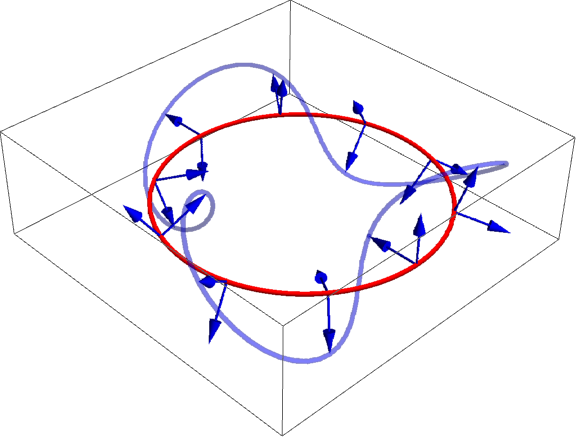
\includegraphics[width=5cm]{twistedDNA2.png}}\quad\subfloat[]{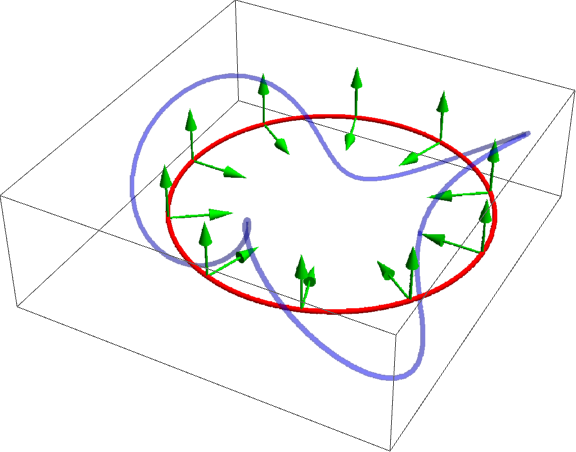
\includegraphics[width=5cm]{twistedDNA1.png}}
\caption{\label{minicircledna}Depictions of a possible minicircle DNA model.  (a) The red circle is the tube's axis. The blue curve represents the tip of the vector $\v{d}_1$ and indicates the extend to which the tube is twisted. (b) the green vectors represent the twist free basis $({\bf E}_1,{\bf E}_2)$.}
\end{figure}
Consider a simple model for a DNA mini-circle as a twisted elastic tube. The tube's axis is assumed to be a circle
\begin{equation}
\v{r}(t) = \left(R\cos(2\pi t),R\sin(2\pi t),0\right), t\in[0,1]
\end{equation}
where $R$ is the radius of the circle. We assume tube can be modelled as an unstretchable tube satisfying the folowing kinematic equations
\begin{equation}
\label{stretchkinematics}
\fd{}{s}
\left(\begin{array}{c} \v{r} \\ \v{d}_1 \\\v{d}_2\\ \v{d}_3 \end{array}\right) = 
\left(\begin{array}{cccc}
0 &0 & 0 & 1\\
0 & 0 &  u_3 & -u_2\\
0 & -u_3 &  0 & u_1\\
0 & u_2 &  -u_1 & 0
\end{array}\right)
\left(\begin{array}{c}\v{r}\\ \v{d}_1 \\ \v{d}_2 \\ \v{d}_3 \end{array}\right).
\end{equation}
and the following equilibrium equations
\begin{align}
\label{mechanics2}
\fd{}{s}\v{n}&= {\bf 0},\\
\nonumber \fd{}{s}\v{m}  +\v{d}_3 \times\v{n} &={\bf 0}.
\end{align}
where $\v{n}$ is the internal force of the tube, $\v{m}$ the internal couple. We assume the following constitutive laws for the system
\begin{equation}
\v{m} = A u_1\v{d}_1 + B u_2{\bf  d}_2 + C u_3\v{d}_3,\quad \v{n} = n_1\v{d}_1 + n_2\v{d}_2 +  n_3\v{d}_3.
\end{equation}
\begin{enumerate}[label=(\alph*)]
\item{Find the arclength parametrsiation $\v{r}(s)$ of this curve.
}
\item{Express the $\v{d}_i$ components of the equations (\ref{mechanics2}).
}
\item{
It can be shown that the kinematic parameters can be written as
\begin{equation}
u_1 = \frac{\sin(\phi(s))}{R},\quad u_2=\frac{\cos(\phi(s))}{R},\quad u_3 = \fd{\phi}{s}.
\end{equation}
If $\phi(s)=0,\forall s$ then the pair $(\v{d}_1,\v{d}_2)$ are parallel transported around  $\v{r}(s)$, as shown in Figure \ref{minicircledna}(b), this represents an untwisted tube. An example of a non zero twisted tube (basis pair) is shown in Figure \ref{minicircledna}(a). State the (two) boundary conditions on $\phi$ on the assumption that the deformation of the tube is differentiable.
}\item{
Demonstrate that the twist function $\fd{\phi}{s}$ takes the following implict form:
\begin{equation}
\fd{\phi}{s}=\pm \sqrt{2\left(D+\frac{\cos(2\phi)}{4R^2}(B-A)\right)/C},
\end{equation}
where $D$ is a constant of integration.
}\item{
Find a condition on the constants $A$ and $B$ for the possibility of solutions to the full system of equations when there is non-zero twisting. You may assume that the O.D.E for $\phi$ obtained in the previous question has solutions. (Hint: you should not need to solve the equations).
}
\end{enumerate}
\section{}
The kinematics of the rod  are described by the set of vectors $\v{r}(s),\v{d}_i(s)[0,L]\rightarrow \mathbb{R}^3\,,i=1,2,3$ and the following system of ordinary differential equations
\begin{equation*}
\label{fullkinematics}
\fd{}{s}
\left(\begin{array}{c} \v{r} \\ \v{d}_1 \\\v{d}_2\\ \v{d}_3 \end{array}\right) = 
\left(\begin{array}{cccc}
0 &0 & 0 & \nu \\
0 & 0 &  u_3 & -u_2\\
0 & -u_3 &  0 & u_1\\
0 & u_2 &  -u_1 & 0
\end{array}\right)
\left(\begin{array}{c}\v{r}\\ \v{d}_1 \\ \v{d}_2 \\ \v{d}_3 \end{array}\right),
\end{equation*}
with the $u_i,\nu$ smooth scalar functions of $s$ representing the system's curvatures and stretching

The equations of equilibrium of this body are given by the following vector equations:
\begin{align}
\label{mechanics}
\fd{}{s}\v{n}&= {\bf 0},\\
\nonumber \fd{}{s}\v{m}  +\fd{\v{r}}{s}\times\v{n} &={\bf 0}.
\end{align}
The following choice of constitutive law for the internal couple is assumed
\begin{equation*}
\v{m} =  A u_1\v{d}_1 + A u_2\v{d}_2 +C u_3\v{d}_3,
\end{equation*}
with $A,C>0$ constants. To complete the system (\ref{mechanics}) we assume the following consttutive law relating the axial force and the stretching:
\begin{equation}
n_3(s) = E(\nu(s)-1).
\end{equation}
where $E$ is the Young's modulus of the elastic rod. 
\begin{enumerate}[label=(\alph*)]
\item{Write out the system (\ref{mechanics}) in component form in the $(\v{d}_1,\v{d}_2,\v{d}_3)$ basis.

}\item{Now assume that $u_2=u_3=0$, how does this constraint the tube's geometry?
}\item{Use the assumption that $u_2=u_3=0$ to reduce the system (\ref{mechanics}) to a pair of non-linear ordinary differential equations for $\nu$ and $u_1$.
}\item{Verify that a straight vertical rod with arbitrary \emph{constant compression} is in equilibrium for this model and given an expression for the compression under an axial load $N$ applied to the rod.
}\item{Demonstrate the rod is unstable to the forces with the following values for integer $n$: 
\begin{equation}
N =\frac{1}{2} \left(E \pm \sqrt{E}\sqrt{E-\frac{4 \pi ^2 A n^2}{L^2}} \right)
\end{equation} 
To do this assume the rod remains planar under small perturbations about this equilibrium (Hint: perform a linear stability analysis). 
}\end{enumerate}


\section{}

\begin{figure}
\centering
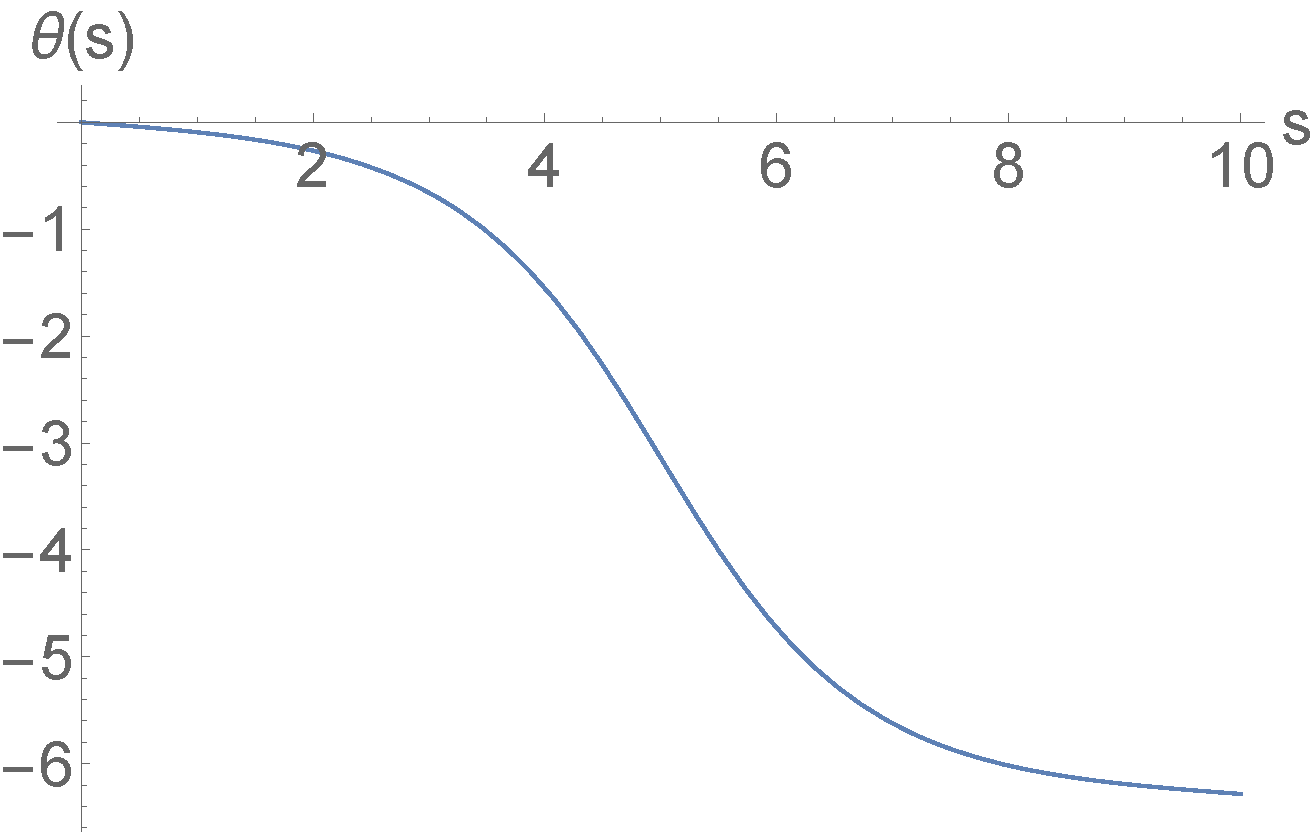
\includegraphics[width=8cm]{thetaPlot.pdf}
\caption{\label{q1fig} A function $\theta(s),\, s\in[0,10]$ which is a solution to the tube system considered in Question 5}
\end{figure}
Consider a slender elastic rod whose central axis is represented by a curve $\v{r}(s):[0,L]\rightarrow \mathbb{R}^3$, where $s$ is the body's arclength. The coordinates of $\mathbb{R}^3$ take the form $(x,y,z)$ with unit vectors $\uv{x},\uv{y}$ and $\uv{z}$ respectively. A force $\v{n}(s)$ represents the internal force acting on each cross-section of the the body and $\v{m}(s)$ represents the internal couple acting on each cross section. Net forces and couples can be applied at $s=0$ and $s=L$. 

The kinematics of the rod  are described by the set of vectors $\v{r}(s),\v{d}_i(s):[0,L]\rightarrow \mathbb{R}^3\,,i=1,2,3$ and the following system of ordinary differential equations
\begin{equation*}
\label{fullkinematics}
\fd{}{s}
\left(\begin{array}{c} \v{r} \\ \v{d}_1 \\\v{d}_2\\ \v{d}_3 \end{array}\right) = 
\left(\begin{array}{cccc}
0 &0 & 0 & 1 \\
0 & 0 &  u_3 & -u_2\\
0 & -u_3 &  0 & u_1\\
0 & u_2 &  -u_1 & 0
\end{array}\right)
\left(\begin{array}{c}\v{r}\\ \v{d}_1 \\ \v{d}_2 \\ \v{d}_3 \end{array}\right),
\end{equation*}
with the $u_i$ smooth scalar functions of $s$ representing the system's curvatures.

The equations of equilibrium of this body are given by the following vector equations:
\begin{align}
\label{mechanics}
\fd{}{s}\v{n}&= {\bf 0},\\
\nonumber \fd{}{s}\v{m}  +\v{d}_3 \times\v{n} &={\bf 0}.
\end{align}
The following choice of constitutive law for the internal couple is assumed
\begin{equation*}
\v{m} =  A u_1\v{d}_1 + A u_2\v{d}_2 +C u_3\v{d}_3,
\end{equation*}
with $A,C>0$ constants. Further assume the rod is a planar curve and the pair  $\v{d}_3$ and $\v{d}_1$ are parameterised by a function $\theta(s)$:
\begin{equation*}
\v{d}_3(s) = \left(\cos\theta(s),0,\sin\theta(s)\right),\quad \v{d}_1(s) = \left(-\sin\theta(s),0,\cos\theta(s)\right).
\end{equation*} 
Assume the rod is never twisted ($u_3=0$). Finally, consider the rod to be attached to a wall at $s=0$ at an angle $\theta=0$ and that a load $N \uv{x}$ pushing on the rod is applied at $s=L$.
\begin{enumerate}[label=(\alph*)]
\item{Show that the system (\ref{mechanics}) can be reduced to the following non-linear ODE for $\theta$:
\begin{equation}
\label{maineq}
A\fdd{\theta}{s} -N\sin(\theta)=0.
\end{equation} 
}\item{
Using the following integral identity 
\begin{equation*}
\int^{\theta}\frac{\d\theta}{\sqrt{C_1-\gamma\cos\theta}} = \frac{2}{\sqrt{C_1-\gamma}} F\left(\frac{\theta}{2}\large\bigg \vert \frac{2 \gamma}{C_1-\gamma}\right),
\end{equation*}
where 
\begin{equation*}
F\left(x\large\vert k\right) = \int_{0}^{x}\frac{\d x'}{\sqrt{1-k^2\sin^2 x'}}
\end{equation*}
is the elliptic integral of the first kind, integrate (\ref{maineq}) twice in order to find an implicit relationship between $\theta$ and $s$ and  a constant of integration $C_1$. In doing so you  should impose the stated boundary condition on $\theta$ at $s=0$. 
}\item{
State a constraint on the value of $C_1$ in terms of the applied load $N$ and bending stiffness $A$.
}\item{
The elliptic integral of the first kind has an inverse, the so-called Jacobi amplitude function $\mathrm{am}(x\vert k)$ defined by
\begin{equation*}
F\left(\mathrm{am}(x\vert k)\large\vert k\right) = x.
\end{equation*}
Use this relation to obtain an explicit solution for $\theta$.
}\item{An example solution for $\theta(s),s\in[0,10]$ is shown in Figure \ref{q1fig}. Describe/sketch the tube configuration $\v{r}(s),s\in[0,10]$ corresponding to this solution. Is it physically realistic? } 
\item{Consider a similar model except with the bending coefficient $A(s)$ dependent on the arclength. What does this represent physically and how would it alter the equation obtained in (a) (assuming all else stays equal)? }
\end{enumerate}

\end{document}
